% Classic paper style
\documentclass[12pt]{article}
\usepackage[a4paper,left=2.5cm,right=2.5cm]{geometry}

% Set wide A4 format
\usepackage{a4wide}

% Support for Czech alphabet
\usepackage[czech]{babel}
\usepackage[utf8]{inputenc}
\usepackage{graphicx}
\usepackage{caption}
\usepackage{subcaption}

% Document beginning
\begin{document}

% Title page
\title{SSU 05 – Ensembling}
\author{Lukáš Hromadník}
\date{}

\pagestyle{empty}
\maketitle
\thispagestyle{empty}

\pagestyle{plain}

% Content

\section{Assignment 1}

\begin{figure}[!h]
    \centering
    \begin{subfigure}[b]{0.49\textwidth}
        \centering
        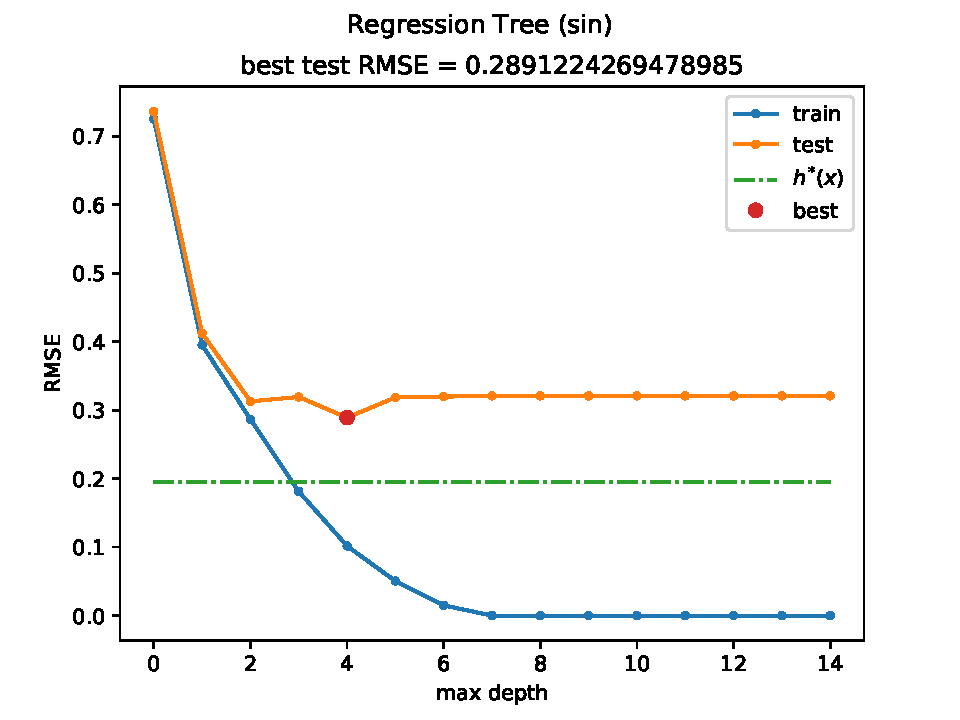
\includegraphics[width=0.9\textwidth]{plots/01/regression_tree_sin.pdf}
        \caption{Sin dataset}
        \label{fig:01-sin}
    \end{subfigure}
    \begin{subfigure}[b]{0.49\textwidth}
        \centering
        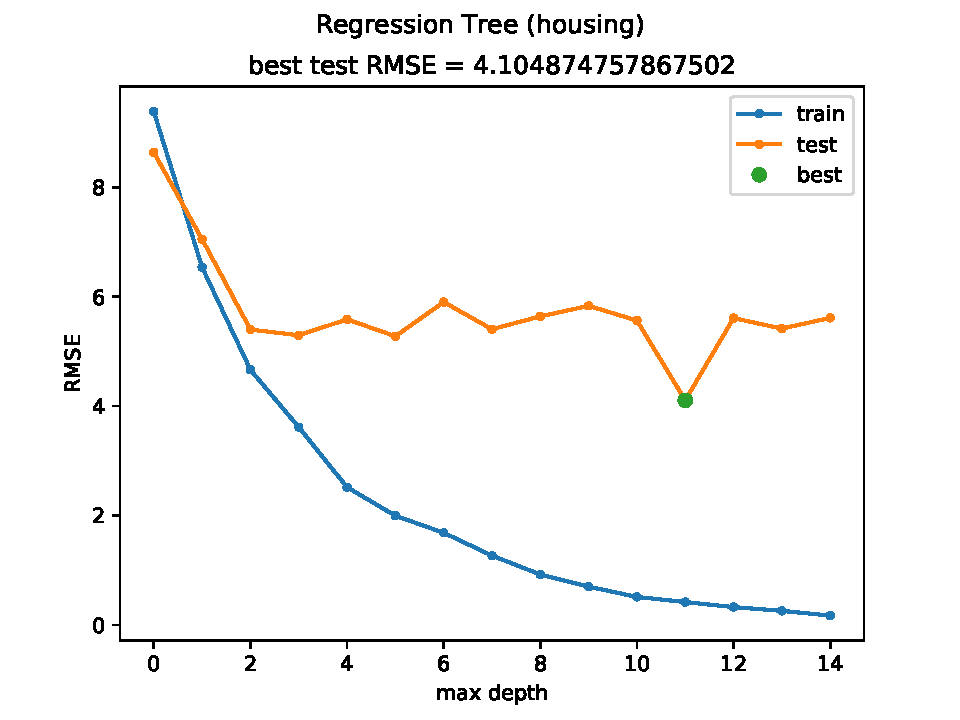
\includegraphics[width=0.9\textwidth]{plots/01/regression_tree_housing.pdf}
        \caption{Boston housing dataset}
        \label{fig:01-housing}
    \end{subfigure}
    \caption{Assignment 1 results}
\end{figure}

The figure \ref{fig:01-sin} in which sin dataset is plotted shows that the optimal depth for the tree to grow is 3. From the depth of 7 and more the tree overfits training data and cannot improve itself. Overfitting is visible on the test data too. The error on the test data is the same from a depth of 7.

The Boston housing dataset in figure \ref{fig:01-housing} has more parameters to learn. In the result we can see that the optimal depth has value of 11. The maximal depth in this example was not enough to overfit the given data. There is a noticaeble trend that in a deeper tree the classifier will overfit the data.

\newpage

\section{Assignment 2}

\begin{figure}[!h]
    \centering
    \begin{subfigure}[b]{0.49\textwidth}
        \centering
        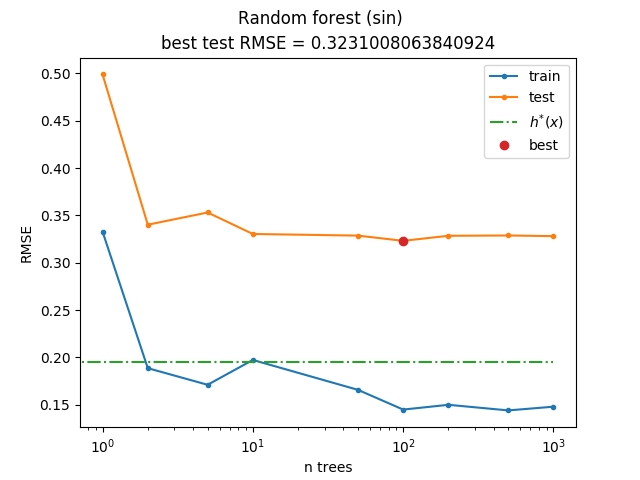
\includegraphics[width=0.9\textwidth]{plots/02/01-sin.png}
        \caption{Sin dataset}
        \label{fig:02-sin}
    \end{subfigure}
    \begin{subfigure}[b]{0.49\textwidth}
        \centering
        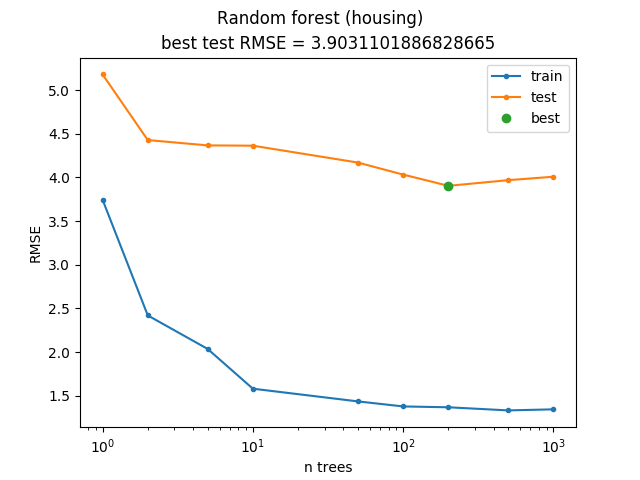
\includegraphics[width=0.9\textwidth]{plots/02/02-housing.png}
        \caption{Boston housing dataset}
        \label{fig:02-housing}
    \end{subfigure}
    \begin{subfigure}[b]{0.49\textwidth}
        \centering
        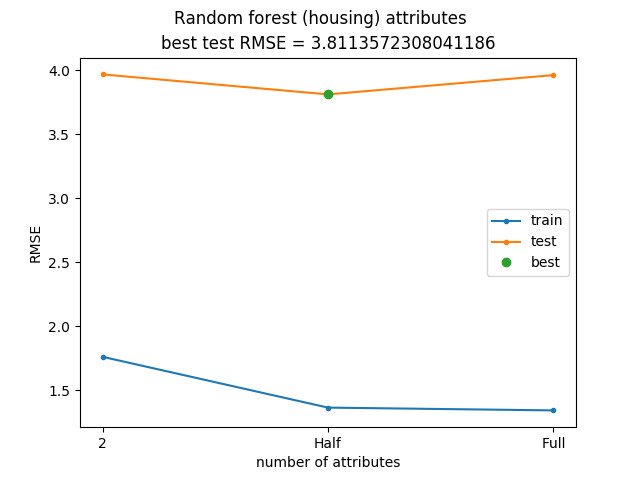
\includegraphics[width=0.9\textwidth]{plots/02/03-attributes.png}
        \caption{Number of attributes used for learning}
        \label{fig:02-attributes}
    \end{subfigure}
    \caption{Assignment 2 results}
\end{figure}

From the first figure \ref{fig:02-sin} it is clear that optimal number of trees in Random forest learned on a sin dataset is 100. Another interesting thing is that adding more trees to the forest doesn't improve final result.

Second figure \ref{fig:02-housing} shows housing dataset. The optimal number of trees for this dataset is 200. Same thing as in the previous result appeared here that more trees don't improve the final result.

Last figure \ref{fig:02-attributes} shows performance given a number of attributes to learn in the tree. Best result is given by using half of the attributes from the dataset.

\newpage

\section{Assignment 3}

\begin{figure}[!h]
    \centering
    \begin{subfigure}[b]{0.49\textwidth}
        \centering
        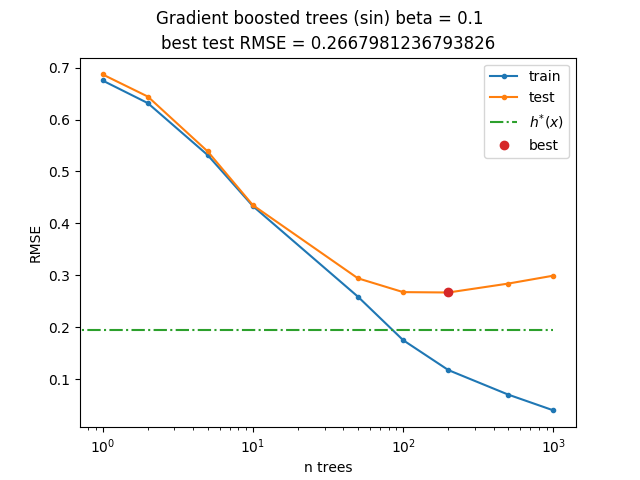
\includegraphics[width=0.9\textwidth]{plots/03/01-sin-0-1.png}
        \caption{$\beta = 0.1$}
        \label{fig:03-sin-0.1}
    \end{subfigure}
    \begin{subfigure}[b]{0.49\textwidth}
        \centering
        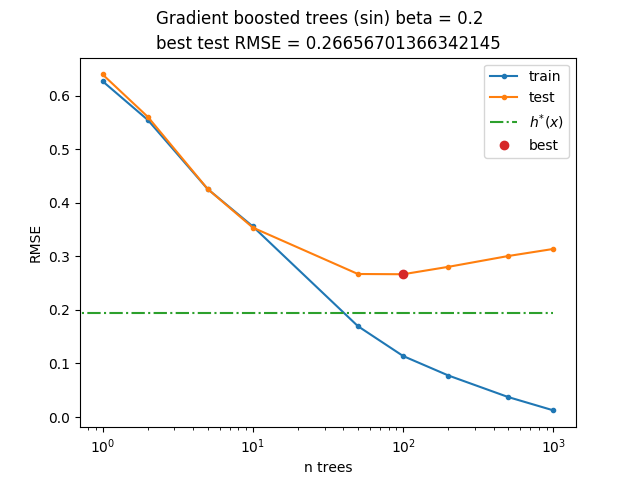
\includegraphics[width=0.9\textwidth]{plots/03/01-sin-0-2.png}
        \caption{$\beta = 0.2$}
        \label{fig:03-sin-0.2}
    \end{subfigure}
    \begin{subfigure}[b]{0.49\textwidth}
        \centering
        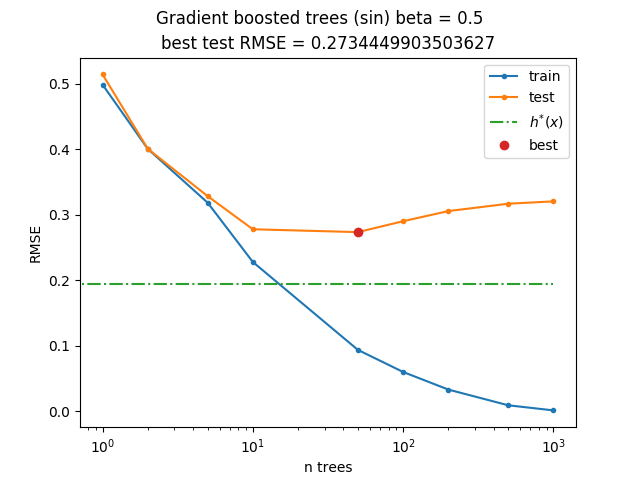
\includegraphics[width=0.9\textwidth]{plots/03/01-sin-0-5.png}
        \caption{$\beta = 0.5$}
        \label{fig:03-sin-0.5}
    \end{subfigure}
    \begin{subfigure}[b]{0.49\textwidth}
        \centering
        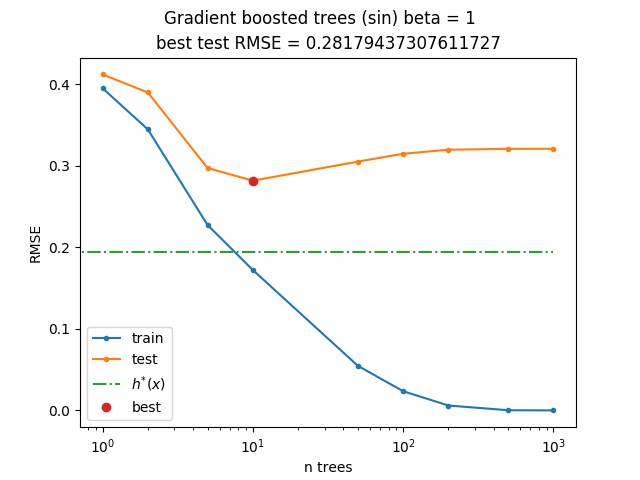
\includegraphics[width=0.9\textwidth]{plots/03/01-sin-1.png}
        \caption{$\beta = 1$}
        \label{fig:03-sin-1}
    \end{subfigure}
    \caption{Assignment 3 Sin dataset results}
    \label{fig:03-sin}
\end{figure}

There are four graphs in \ref{fig:03-sin} depicting learning of Gradient boosted trees with different parameter $\beta$ given sin dataset. The best result is given by $\beta = 0.2$ and it's RMSE = $0.2666$. Another thing that can be seen from the graphs is that with increasing value of $\beta$ the number of trees needed for the best value is decreasing.

\newpage

\begin{figure}[!h]
    \centering
    \begin{subfigure}[b]{0.49\textwidth}
        \centering
        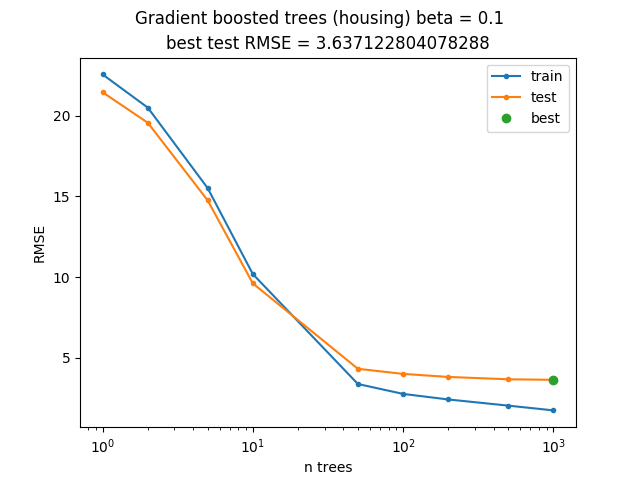
\includegraphics[width=0.9\textwidth]{plots/03/02-housing-0-1.png}
        \caption{$\beta = 0.1$}
        \label{fig:03-housing-0.1}
    \end{subfigure}
    \begin{subfigure}[b]{0.49\textwidth}
        \centering
        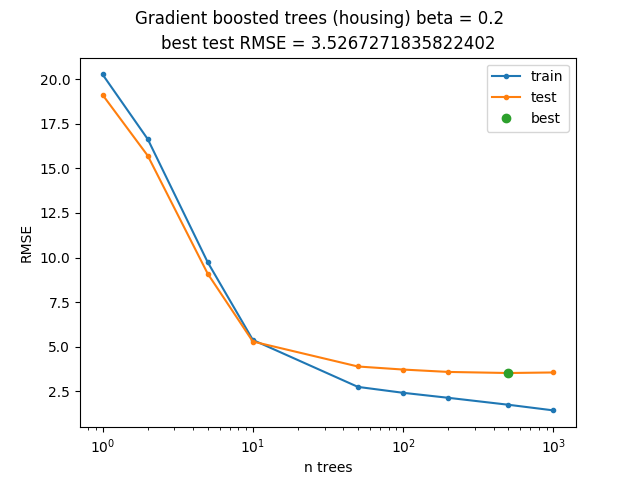
\includegraphics[width=0.9\textwidth]{plots/03/02-housing-0-2.png}
        \caption{$\beta = 0.2$}
        \label{fig:03-housing-0.2}
    \end{subfigure}
    \begin{subfigure}[b]{0.49\textwidth}
        \centering
        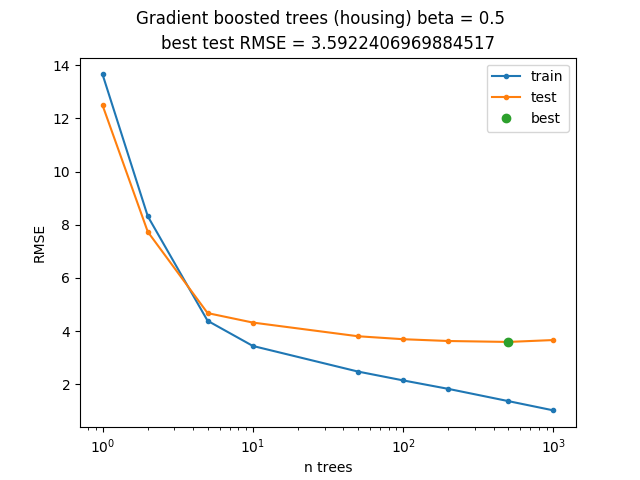
\includegraphics[width=0.9\textwidth]{plots/03/02-housing-0-5.png}
        \caption{$\beta = 0.5$}
        \label{fig:03-housing-0.5}
    \end{subfigure}
    \begin{subfigure}[b]{0.49\textwidth}
        \centering
        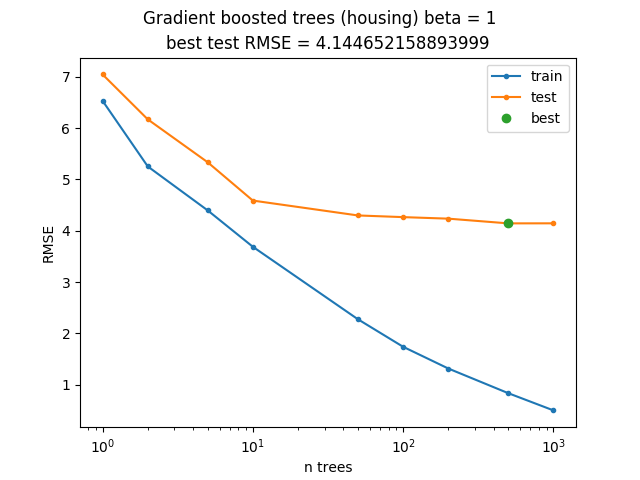
\includegraphics[width=0.9\textwidth]{plots/03/02-housing-1.png}
        \caption{$\beta = 1$}
        \label{fig:03-housing-1}
    \end{subfigure}
    \caption{Assignment 3 Housing dataset results}
    \label{fig:03-housing}
\end{figure}

Gradient boosted trees results given housing dataset in figure \ref{fig:03-housing} are more or less the same. The best result is given by $\beta = 0.2$ and it's RMSE = $3.5267$. Here with the increasing value of $\beta$ the number of trees used in for the best value doesn't decrease. That's probably because the dataset is more complex than the previous one.

\newpage 

\section{Assignment 4}

\begin{center}
\begin{tabular}{|l|c|}
    \hline
    Number of threads & Duration time \\ \hline
    1 & 500.25 s \\ \hline
    4 & 148.00 s \\ \hline
    6 & 142.65 s \\ \hline
    8 & 143.83 s \\ \hline
\end{tabular}
\end{center}

The best result is given with 6 threads. This result was measured on the 4-core / 8 threads system. Using the same number of threads for computation as the maximal number of threads for the CPU isn't the best choice because there is always at least one thread (the main thread) which is used by the system. That's the reason why in my case it was the best to use 6 threads.

The implementation is available inside the \verb|RandomForest| class.

% End of document
\end{document}
